\documentclass[11pt]{amsart}
\usepackage[utf8]{inputenc}
\usepackage{xcolor}
\usepackage{amsmath,amssymb,amsthm}
\usepackage{graphicx}
\usepackage{booktabs}
\usepackage{microtype}
\setlength{\emergencystretch}{2em}
\usepackage[margin=1in]{geometry}
\usepackage[colorlinks=true,linkcolor=blue!50!black,citecolor=blue!50!black,urlcolor=blue!50!black]{hyperref}

\newtheorem{theorem}{Theorem}
\renewcommand{\thetheorem}{\Alph{theorem}}
\newtheorem{lemma}{Lemma}[section]
\newtheorem{proposition}[lemma]{Proposition}
\newtheorem{corollary}[lemma]{Corollary}
\theoremstyle{remark}
\newtheorem{remark}[lemma]{Remark}
\theoremstyle{definition}
\newtheorem{definition}[lemma]{Definition}

\newcommand{\Lam}{\Lambda}
\newcommand{\gE}{\gamma_E}
\newcommand{\dd}{\,\mathrm{d}}
\renewcommand{\Re}{\operatorname{Re}}
\renewcommand{\Im}{\operatorname{Im}}

\title[A double-pole mean square and simple zeros]{A mean square with double poles at the zeros of $\zeta$: \\ the rightmost zero, a Cram\'er-type asymptotic, \\ and a criterion for simple zeros}
\author{Vincent P.\,P. No\"el}
\address{Strasbourg, France}
%\email{}   % to be completed by the author
\date{October 2026. Preprint, not peer reviewed.}
\subjclass[2020]{Primary 11M26; Secondary 11N05, 40E05}
\keywords{Riemann zeta function, mean square, Cram\'er's theorem, simple zeros, Nyman--Beurling criterion}

\begin{document}

\begin{abstract}
Let $c=\Lam*\Lam-\Lam\cdot\log+2\gE\Lam$, $C(x)=\sum_{n\le x}c(n)$ and $Q(X)=\int_1^X|C(x)|^2x^{-2}\dd x$. The Dirichlet series of $c$ is $G=q^2+q'+2\gE q$ with $q=-\zeta'/\zeta$; it is regular at $s=1$ and has a double pole with leading coefficient $m(m+1)$ at every non-trivial zero of multiplicity $m$. We show: (A) unconditionally, $\tfrac12\limsup_{X\to\infty}\log(1+Q(X))/\log X=\Theta-\tfrac12$, where $\Theta$ is the supremum of the real parts of the zeros; (B) under the Riemann Hypothesis, $Q(X)\sim\tfrac{S}{3}(\log X)^3$ with $S=\sum_{\rho\ \mathrm{distinct}}m(\rho)^2(m(\rho)+1)^2/|\rho|^2$; and (B$'$) under RH, $S\ge 4\kappa$ with equality if and only if all zeros are simple, where $\kappa=2+\gE-\log 4\pi$. Thus, under RH, $Q(X)/(\log X)^3\to 4\kappa/3$ if and only if all zeros are simple. Combining (A) and (B$'$), the same limit characterises the conjunction of RH and simplicity without assuming RH in advance. We also record an exact identity linking $Q$ to a two-parameter family in the Nyman--Beurling--B\'aez-Duarte criterion, and numerical checks up to $X=10^8$. Part (A) uses a standard method and part (B) is the double-pole analogue of Cram\'er's mean-square theorem; no progress towards the Riemann Hypothesis is claimed.
\end{abstract}

\maketitle

\section{Introduction}

Classical equivalents of the Riemann Hypothesis (RH), such as $\psi(x)=x+O(x^{1/2+\varepsilon})$, compare the size of an arithmetic sum with the position of the zeros. The mean-square form goes back to Cram\'er~\cite{Cra22}: under RH,
\begin{equation}\label{eq:cramer}
\int_1^X\frac{(\psi(x)-x)^2}{x^2}\dd x\sim c_1\log X,\qquad c_1=\sum_{\rho\ \mathrm{distinct}}\frac{m(\rho)^2}{|\rho|^2},
\end{equation}
see Montgomery--Vaughan~\cite[Thm.~13.6]{MV07} and Brent--Platt--Trudgian~\cite[eq.~(18)]{BPT22}, who also study the mean square of $\psi(x)-x$ over dyadic intervals.

This note studies a variant in which the underlying Dirichlet series has a \emph{double} pole at each zero and no singularity at $s=1$. Write $q(s)=-\zeta'(s)/\zeta(s)=\sum_{n\ge1}\Lam(n)n^{-s}$ and
\[
c(n)=(\Lam*\Lam)(n)-\Lam(n)\log n+2\gE\Lam(n),\qquad G(s)=\sum_{n\ge1}c(n)n^{-s}=q^2+q'+2\gE q,
\]
\[
C(x)=\sum_{n\le x}c(n),\qquad Q(X)=\int_1^X\frac{|C(x)|^2}{x^2}\dd x .
\]
The choice of $c$ is dictated by two requirements: $q^2+q'$ has a double pole with coefficient $m(m+1)\neq0$ at each zero of multiplicity $m$, and the term $2\gE q$ removes the singularity at $s=1$, so that no main term has to be subtracted from $C$. The function $c$ is supported on integers with at most two distinct prime factors (Lemma~\ref{lem:support}).

\subsection*{Results} Let $\Theta=\sup\{\Re\rho\}$, the supremum over the non-trivial zeros, and $\kappa=2+\gE-\log4\pi=0.0461914179\ldots$

\begin{theorem}[standard method]\label{thm:A}
Unconditionally,
\[
\tfrac12\limsup_{X\to\infty}\frac{\log(1+Q(X))}{\log X}=\Theta-\tfrac12 .
\]
In particular RH holds if and only if $Q(X)=X^{o(1)}$; and for $0\le\delta\le\tfrac12$, $Q(X)\ll_\varepsilon X^{2\delta+\varepsilon}$ for every $\varepsilon>0$ if and only if $\Theta\le\tfrac12+\delta$.
\end{theorem}

\begin{theorem}\label{thm:B}
Assume RH. Put $A_\rho=m(\rho)(m(\rho)+1)$ and $S=\sum_{\rho\ \mathrm{distinct}}A_\rho^2/|\rho|^2$. Then $S<\infty$ and
\[
Q(X)\sim\frac S3(\log X)^3\qquad(X\to\infty).
\]
If all zeros are simple, then $S=4\kappa$ and $Q(X)\sim\frac{4\kappa}{3}(\log X)^3$.
\end{theorem}

\begin{corollary}\label{cor:Bprime}
Assume RH. Then $S\ge4\kappa$, with equality if and only if every non-trivial zero of $\zeta$ is simple. Consequently, under RH,
\[
\lim_{X\to\infty}\frac{Q(X)}{(\log X)^3}=\frac{4\kappa}{3}\iff\text{all zeros of }\zeta\text{ are simple.}
\]
\end{corollary}

\begin{corollary}[Joint criterion for RH and simplicity]\label{cor:joint}
Without assuming RH in advance,
\[
\lim_{X\to\infty}\frac{Q(X)}{(\log X)^3}=\frac{4\kappa}{3}
\iff \text{RH holds and every non-trivial zero of }\zeta\text{ is simple.}
\]
\end{corollary}
\begin{proof}
The stated finite limit implies $Q(X)=O((\log X)^3)$, so Theorem~\ref{thm:A} gives $\Theta=\frac12$, hence RH. Corollary~\ref{cor:Bprime} then gives simplicity. Conversely, RH and simplicity give the stated limit by Theorem~\ref{thm:B}. This combines the preceding results; it supplies no independent proof of RH or simplicity.
\end{proof}

Theorem~\ref{thm:A} is the mean-square analogue, for $G$, of the classical characterisation of $\Theta$ through $\psi(x)-x$ (\cite[Ch.~13 and 15]{MV07}); both directions use textbook methods and we do not claim novelty for it. Theorem~\ref{thm:B} is proved by Cram\'er's method (Mellin--Plancherel, local analysis at the poles, a Tauberian step). We have not found it stated in the literature, but a specialist will regard it as the double-pole transposition of~\eqref{eq:cramer}; its interest lies in the explicit constant $S$ with multiplicities and in Corollary~\ref{cor:Bprime}. The same argument applied to~\eqref{eq:cramer} gives the companion statement $c_1\ge\kappa$, with equality if and only if all zeros are simple (Remark~\ref{rem:twin}); the double pole makes the constant more sensitive to multiple zeros (a double zero weighs $4.5$ times as much as two simple zeros at the same place in $S$, against twice as much in $c_1$).

\subsection*{Related work} Generalised von Mangoldt functions $\Lam_k=\mu*\log^k$ and $k$-fold convolutions $\Lam^{*k}$ give RH-equivalent asymptotics for twisted sums (Banks--Sinha~\cite{BS22}; see also Gonek--Graham--Lee~\cite{GGL20}). Our series is not one of theirs: for $\Lam_2$, whose series is $\zeta''/\zeta=q^2-q'$, the double-pole coefficient is $m(m-1)$, which vanishes at simple zeros. Under RH, the bound $C(x)\ll x^{1/2}\log^5x$ follows from \cite[Thm.~1.1]{BS22} with $k=2$ together with classical estimates; no mean square appears there. A $B^2$-almost-periodic framework such as that of Akbary--Ng--Shahabi~\cite{ANS14} could plausibly yield Theorem~\ref{thm:B} once the truncated explicit formula is controlled in mean square; the Plancherel--Tauber route used here avoids that step. Recent unconditional work shows that more than two thirds of the zeros are simple and on the critical line~\cite{AF26,Lam26}; none of it is used below.

\subsection*{Organisation} Section~\ref{sec:G} collects the properties of $G$. Section~\ref{sec:A} proves Theorem~\ref{thm:A}, Section~\ref{sec:B} Theorem~\ref{thm:B}, Section~\ref{sec:Bprime} Corollary~\ref{cor:Bprime}; the joint criterion (Corollary~\ref{cor:joint}) follows directly from (A) and (B$'$). Section~\ref{sec:NB} gives an exact identity relating $Q$ to the Nyman--Beurling--B\'aez-Duarte criterion. Section~\ref{sec:num} reports numerical checks, and Section~\ref{sec:open} lists open questions.

\section{The series $G$}\label{sec:G}

Throughout, $\rho=\beta+i\gamma$ runs over the non-trivial zeros of $\zeta$, counted with multiplicity $m(\rho)$ unless ``distinct'' is specified, and $s=\sigma+it$. Implied constants may depend on $\varepsilon$ and on $\zeta$, never on $x$, $X$ or $t$.

\begin{lemma}\label{lem:gen}
For $\Re s>1$, $G=q^2+q'+2\gE q$. Moreover, with $f=1/\zeta$ and $a(n)=\mu(n)(\log^2n-2\gE\log n)$, one has $G=\zeta\cdot(f''+2\gE f')$ and $c=1*a$.
\end{lemma}
\begin{proof}
$q^2$ is the series of $\Lam*\Lam$ and $q'=-\sum\Lam(n)\log n\,n^{-s}$. Since $f'=fq$ and $f''=fq^2+fq'$, we get $\zeta(f''+2\gE f')=q^2+q'+2\gE q$, and $f''+2\gE f'=\sum a(n)n^{-s}$.
\end{proof}

\begin{lemma}\label{lem:support}
$c(p^k)=-\log^2p+2\gE\log p$; $c(p^ar^b)=2\log p\log r$ for distinct primes $p\ne r$ and $a,b\ge1$; and $c(n)=0$ if $n$ has at least three distinct prime factors. Hence $|c(n)|\ll\log^2n$ and $\sum_n|c(n)|n^{-\sigma}\ll(\sigma-1)^{-2}$ as $\sigma\to1^+$.
\end{lemma}
\begin{proof}
$(\Lam*\Lam)(p^k)=(k-1)\log^2p$ and $(\Lam*\Lam)(p^ar^b)=2\log p\log r$; $\Lam*\Lam$ vanishes on integers with three or more prime factors. The last bound follows from $\sum|c(n)|n^{-\sigma}\le q(\sigma)^2+|q'(\sigma)|+2\gE q(\sigma)$.
\end{proof}

\begin{lemma}\label{lem:one}
$G$ is holomorphic at $s=1$, with $G(1)=2\gE^2+6\gamma_1$.
\end{lemma}
\begin{proof}
From $q=(s-1)^{-1}-\gE+O(s-1)$ we get $q^2=(s-1)^{-2}-2\gE(s-1)^{-1}+O(1)$, $q'=-(s-1)^{-2}+O(1)$ and $2\gE q=2\gE(s-1)^{-1}+O(1)$: the polar parts cancel.
\end{proof}

\begin{lemma}\label{lem:poles}
Let $\rho$ be a non-trivial zero of multiplicity $m$, and write $q=-m/(s-\rho)+q_0+O(s-\rho)$. Then
\[
G(s)=\frac{m(m+1)}{(s-\rho)^2}+\frac{b_\rho}{s-\rho}+O(1),\qquad b_\rho=-2m(q_0+\gE).
\]
For a simple zero, $b_\rho=\zeta''(\rho)/\zeta'(\rho)-2\gE$. Each trivial zero $-2k$ is a double pole with leading coefficient $2$, and $G$ is regular at $s=0$.
\end{lemma}
\begin{proof}
Direct expansion of $q^2+q'+2\gE q$.
\end{proof}

\begin{lemma}[Mellin identity]\label{lem:mellin}
For $\Re s>1$, $G(s)/s=\int_1^\infty C(x)x^{-s-1}\dd x$.
\end{lemma}
\begin{proof}
Partial summation, using $C(X)\ll X\log^2X$ from Lemma~\ref{lem:support}.
\end{proof}

Since $c(1)=0$ and $c(2)=\log2\,(2\gE-\log2)\approx0.320$, $Q(X)=0$ for $X\le2$ and $Q(X)>0$ for $X>2$; $Q$ is continuous and non-decreasing.

\section{Proof of Theorem~\ref{thm:A}}\label{sec:A}

We use the following classical inputs.
\begin{itemize}
\item[(F1)] Uniformly for $-1\le\sigma\le2$, $|t|\ge2$: $\zeta'/\zeta(s)=\sum_{|t-\gamma|<1}(s-\rho)^{-1}+O(\log|t|)$, and $\#\{\rho:|\gamma-t|<1\}\ll\log|t|$ \cite[Thms.~9.2, 9.6(A)]{Tit86}, \cite[Ch.~15]{Dav00}.
\item[(F2)] The truncated Perron formula \cite[Lemma~3.12]{Tit86}, \cite[Cor.~5.3]{MV07}: if $F(s)=\sum a_nn^{-s}$ with $a_n=O(\mathcal A(n))$, $\mathcal A$ non-decreasing, and $\sum|a_n|n^{-\sigma}\ll(\sigma-1)^{-\alpha}$ as $\sigma\to1^+$, then for $b>1$, $T\ge2$ and non-integral $x>1$ with nearest integer $N$,
\[
\sum_{n<x}a_n=\frac1{2\pi i}\int_{b-iT}^{b+iT}F(s)\frac{x^s}{s}\dd s+O\Big(\frac{x^b}{T(b-1)^\alpha}\Big)+O\Big(\frac{\mathcal A(2x)x\log x}{T}\Big)+O\Big(\frac{\mathcal A(N)x}{T|x-N|}\Big).
\]
\end{itemize}

\begin{proof}[Proof of the lower bound $\Theta-\frac12\le\lambda$]
Let $\lambda$ denote the left-hand side of Theorem~\ref{thm:A}. By Lemma~\ref{lem:support}, $|C(x)|\ll x\log^2x$, so $Q(X)\ll X\log^4X$ and $0\le\lambda\le\frac12$; if $\lambda=\frac12$ there is nothing to prove since $\Theta\le1$. Assume $\lambda<\frac12$ and fix $a\in(\lambda,\frac12)$. Since $Q$ is non-decreasing, $Q(X)\le KX^{2a}$ for all $X\ge1$. For $k\ge0$, Cauchy--Schwarz gives
\[
\int_{2^k}^{2^{k+1}}|C(x)|x^{-\sigma-1}\dd x\le\Big(\int_{2^k}^{2^{k+1}}\frac{|C(x)|^2}{x^2}\dd x\Big)^{1/2}\Big(\int_{2^k}^{2^{k+1}}x^{-2\sigma}\dd x\Big)^{1/2}\ll2^{k(a+\frac12-\sigma)} .
\]
Summing over $k$, $F(s)=\int_1^\infty C(x)x^{-s-1}\dd x$ converges absolutely and locally uniformly on $H=\{\Re s>\frac12+a\}$, hence is holomorphic there, and $F=G/s$ on $\Re s>1$ by Lemma~\ref{lem:mellin}. Let $P$ be the (discrete, closed) set of poles of $G/s$ in $H$; $H\setminus P$ is open and connected, and $F-G/s$ vanishes on it by the identity theorem. If a non-trivial zero $\rho$ lay in $H$, then $G/s=F$ would be bounded on a punctured disc around $\rho$, whereas by Lemma~\ref{lem:poles} $G(s)/s=m(m+1)\rho^{-1}(s-\rho)^{-2}+O(|s-\rho|^{-1})$ is unbounded. Hence $\Theta\le\frac12+a$, and letting $a\downarrow\lambda$ gives the claim.
\end{proof}

\begin{proof}[Proof of the upper bound $\lambda\le\Theta-\frac12$]
If $\Theta=1$ this follows from $Q(X)\ll X\log^4X$. Assume $\Theta<1$, fix $0<\varepsilon<1-\Theta$, and put $\sigma_0=\Theta+\varepsilon/2$, $\sigma_1=\Theta+\varepsilon/4$.

\emph{Growth of $G$.} For $\sigma_1\le\sigma\le2$ and $|t|\ge2$ every zero satisfies $\sigma-\beta\ge\varepsilon/4$, so by (F1) $|q(s)|\le(4/\varepsilon)\#\{\rho:|\gamma-t|<1\}+O(\log|t|)\ll_\varepsilon\log|t|$; for $\sigma\ge2$, $|q(s)|\le q(2)$. For $\sigma\ge\sigma_0$ and $|t|\ge3$ the circle $|w-s|=\varepsilon/4$ lies in the region $\{\Re w\ge\sigma_1,|\Im w|\ge2\}$, and Cauchy's formula gives $q'(s)\ll_\varepsilon\log|t|$. Hence $G\ll_\varepsilon\log^2|t|$ on $\{\sigma\ge\sigma_0,|t|\ge3\}$. On the compact set $\{\sigma_0\le\sigma\le2,|t|\le3\}$, $G$ is holomorphic (no zero has $\beta\ge\sigma_0$, and $s=1$ is removable by Lemma~\ref{lem:one}), so $|G|\le M_\varepsilon$ there.

\emph{Perron.} Take $x=N+\frac12$ with $N\ge3$, $b=1+1/\log x$ and $T=x^4$. By Lemma~\ref{lem:support}, (F2) applies to $a_n=c(n)$ with $\mathcal A(n)=K'\log^2(n+2)$ and $\alpha=2$; the three error terms are $\ll x\log^3x/T$. Thus
\[
C(x)=\frac1{2\pi i}\int_{b-iT}^{b+iT}G(s)\frac{x^s}{s}\dd s+O\big(x^{-3}\log^3x\big).
\]

\emph{Contour shift.} $G(s)x^s/s$ is holomorphic on a neighbourhood of the rectangle with vertices $b\pm iT$, $\sigma_0\pm iT$: non-trivial zeros have $\beta\le\Theta<\sigma_0$, $s=1$ is removable, and $s=0$ and the trivial zeros lie in $\Re s\le0$. The left side contributes $\ll x^{\sigma_0}(M_\varepsilon+\int_3^T\log^2t\,\dd t/t)\ll_\varepsilon x^{\sigma_0}\log^3x$, the horizontal sides $\ll x^b\log^2T/T\ll x^{-3}\log^2x$. Hence $C(N+\frac12)\ll_\varepsilon(N+\frac12)^{\Theta+\varepsilon}$; since $C$ is constant on $[N,N+1)$, $|C(x)|\ll_\varepsilon x^{\Theta+\varepsilon}$ for all $x\ge1$.

\emph{Energy.} As $2(\Theta+\varepsilon)-2>-1$, $Q(X)\ll_\varepsilon X^{2\Theta-1+2\varepsilon}$, so $\lambda\le\Theta-\frac12+\varepsilon$ for every $\varepsilon>0$.
\end{proof}

The two consequences stated in Theorem~\ref{thm:A} follow at once (for RH note that $\log(1+Q)/\log X\ge0$, so $\limsup=0$ means $\lim=0$).

\begin{remark}\label{rem:A}
(i) The proof gives the pointwise form $\limsup_{x\to\infty}\log|C(x)|/\log x=\Theta$ and the abscissa form: $\int_1^\infty|C(x)|^2x^{-2\sigma-1}\dd x$ converges for $\sigma>\Theta$ and diverges for $\sigma<\Theta$. At the level of exponents the mean square carries the same information as the pointwise bound; they differ on the logarithmic scale, where Theorem~\ref{thm:B} lives.
(ii) Only the non-vanishing of the polar part of $G$ at each zero is used, not its order. The sign in $q^2+q'$ guarantees it: for $q^2-q'=\zeta''/\zeta$ the leading coefficient is $m(m-1)$, and the same argument would require $\zeta''(\rho)\ne0$ at every simple zero.
(iii) The result is ineffective, and an exponent measured over a finite range says nothing about $\Theta$. Under RH, Theorem~\ref{thm:B} gives
\[
\frac{\log(1+Q(X))}{\log X}
=\frac{3\log\log X+\log(S/3)+o(1)}{\log X}.
\]
At $X=10^7$, the term $3\log\log X/\log X$ alone is about $0.5174$. Under RH and simple zeros, including $\log(4\kappa/3)/\log X$ gives the cubic approximation $0.3445$, compared with the measured $0.325$ in Table~\ref{tab:Q}; the theorem supplies no effective bound on the remaining error at this finite $X$.
\end{remark}

\section{Proof of Theorem~\ref{thm:B}}\label{sec:B}

Assume RH. In addition to (F1) we use:
\begin{itemize}
\item[(F3)] $N(T+1)-N(T)\ll\log T$ \cite[Thm.~9.2]{Tit86}; hence $m(\rho)\ll\log(|\gamma|+2)$ and $\#\{\rho:T<|\gamma|\le2T\}\ll T\log T$.
\item[(F4)] From the Hadamard product \cite[Ch.~12]{Dav00}, for $\Re s\ge\frac12$, $|s-1|\ge\frac12$: $q'(s)=\sum_\rho(s-\rho)^{-2}-(s-1)^{-2}+O(1/|s|)$, the series converging absolutely.
\item[(F5)] (Hardy--Littlewood--Karamata \cite[Ch.~V]{Wid41}, \cite[Ch.~I]{Kor04}.) Let $U:[0,\infty)\to[0,\infty)$ be non-decreasing with $U(0)=0$, and assume $\mathcal LU(\lambda)=\int_{[0,\infty)}e^{-\lambda v}\dd U(v)$ is finite for $\lambda>0$ and $\mathcal LU(\lambda)\sim c\lambda^{-k}$ as $\lambda\downarrow0$. Then $U(L)\sim cL^k/\Gamma(k+1)$.
\end{itemize}

For $\eta>0$ put $Q_\eta=\int_1^\infty|C(x)|^2x^{-2-2\eta}\dd x$ and $U(L)=Q(e^L)$. Let $S_y$ denote $S$ restricted to $|\gamma|\le y$.

\subsection*{Step 1: a priori bound and Plancherel} By the proof of Theorem~\ref{thm:A} with $\Theta=\frac12$, $C(x)\ll_\varepsilon x^{1/2+\varepsilon}$, so $Q(X)\ll_\varepsilon X^{2\varepsilon}$ and $Q_\eta<\infty$ for every $\eta>0$. Fix $\eta\in(0,\frac14]$, $\sigma=\frac12+\eta$, $h(x)=C(x)x^{-\sigma}\mathbf 1_{x\ge1}$. Then $\|h\|^2_{L^2(\dd x/x)}=Q_\eta$, and Cauchy--Schwarz with $Q_{\eta'}$, $0<\eta'<\eta$, shows $h\in L^1(\dd x/x)$. The same estimate shows that $F(s)=\int_1^\infty C(x)x^{-s-1}\dd x$ is holomorphic on $\Re s>\frac12$; it equals $G/s$ on $\Re s>1$, hence on $\Re s>\frac12$ since $G/s$ is holomorphic there under RH (Lemmas~\ref{lem:one}, \ref{lem:poles}). Plancherel (in the variable $\log x$) gives the exact identity
\begin{equation}\label{eq:planch}
Q_\eta=\frac1{2\pi}\int_{\mathbb R}\frac{|G(\sigma+it)|^2}{|\sigma+it|^2}\dd t .
\end{equation}

\subsection*{Step 2: pointwise bound and uniform tail}
\begin{lemma}\label{lem:P}
There is an absolute $K$ such that for $0<\eta\le\frac12$, $\sigma=\frac12+\eta$, $|t|\ge3$,
\[
|G(\sigma+it)|\le K\big[(\log|t|)\,W(t)+\log^2|t|\big],\qquad W(t)=\sum_{|\gamma-t|<1}\frac1{(t-\gamma)^2+\eta^2}.
\]
\end{lemma}
\begin{proof}
Let $Z(t)=\#\{\rho:|\gamma-t|<1\}\ll\log|t|$. Under RH $|s-\rho|^2=\eta^2+(t-\gamma)^2$. By (F1) and Cauchy--Schwarz, $|q(s)|\le(ZW)^{1/2}+O(\log|t|)$. By (F4), $|q'(s)|\le W+\sum_{|\gamma-t|\ge1}(t-\gamma)^{-2}+O(1)$, and splitting the far zeros into unit windows at distance $k\ge1$, each containing $\ll\log(|t|+k)$ zeros, the far sum is $\ll\log|t|$. Since $\sqrt{ZW}\le1+ZW$, $|G|\le|q|^2+|q'|+2\gE|q|\ll(\log|t|)W+\log^2|t|$.
\end{proof}

\begin{lemma}\label{lem:T}
For $Y\ge3$ and $0<\eta\le\frac12$, $\displaystyle\int_{|t|\ge Y}\frac{|G(\sigma+it)|^2}{|\sigma+it|^2}\dd t\le K'\frac{(\log Y)^4}{Y\eta^3}$, with $K'$ absolute.
\end{lemma}
\begin{proof}
By symmetry take $t\ge Y$. Cauchy--Schwarz gives $W(t)^2\le Z(t)\sum_{|\gamma-t|<1}((t-\gamma)^2+\eta^2)^{-2}$, and $\int_{\mathbb R}\dd u/(u^2+\eta^2)^2=\pi/(2\eta^3)$. Hence $\int_T^{2T}W^2\dd t\ll(\log T)\cdot T\log T\cdot\eta^{-3}$ by (F3), and by Lemma~\ref{lem:P} $\int_T^{2T}|G|^2\dd t\ll T(\log T)^4\eta^{-3}$. Using $|s|^{-2}\le T^{-2}$ on $[T,2T]$ and summing over $T=2^jY$ gives the claim.
\end{proof}

Close pairs of zeros are absorbed in the Cauchy--Schwarz step at the cost of one factor $Z\ll\log T$: no information on gaps between zeros is used.

\subsection*{Step 3: local part}
\begin{lemma}\label{lem:loc}
Fix $Y\ge3$. As $\eta\downarrow0$,
\[
\frac{S_{Y-1}}4-o_Y(1)\le\frac{\eta^3}{2\pi}\int_{|t|\le Y}\frac{|G(\sigma+it)|^2}{|\sigma+it|^2}\dd t\le\frac{S_{Y+2}}4+o_Y(1).
\]
\end{lemma}
\begin{proof}
Let $\rho_1,\dots,\rho_J$ be the distinct zeros with $|\gamma_k|\le Y+2$, $A_k=A_{\rho_k}$, $b_k=b_{\rho_k}$, and, if $J\ge2$, $d_Y=\min_{k\ne j}|\gamma_k-\gamma_j|>0$. If $J<2$, the off-diagonal sum below is empty and we set $d_Y=1$ for notation. By Lemmas~\ref{lem:one}, \ref{lem:poles} and RH, $R(s)=G(s)-\sum_k[A_k(s-\rho_k)^{-2}+b_k(s-\rho_k)^{-1}]$ is holomorphic near $K_Y=[\frac12,\frac34]\times[-Y-1,Y+1]$, so $|R|\le M_Y$ there; for $\eta\le\frac14$ the segment $\{\sigma+it:|t|\le Y\}$ lies in $K_Y$. Write $\langle f,g\rangle=\int_{|t|\le Y}f\bar g|s|^{-2}\dd t$, $P_k=A_k(s-\rho_k)^{-2}$, $P=\sum P_k$, $r=G-P$; note $|s|^{-2}\le4$.

(a) \emph{Diagonal.} With $u=t-\gamma_k$, $|P_k|^2=A_k^2(u^2+\eta^2)^{-2}$, and $\big||\sigma+it|^{-2}-|\rho_k|^{-2}\big|\le c_Y(|u|+\eta)$. Using $\eta^3\int_{\mathbb R}(u^2+\eta^2)^{-2}\dd u=\pi/2$, $\eta^3\int_{\mathbb R}|u|(u^2+\eta^2)^{-2}\dd u=\eta$ and $\eta^3\int_{|u|>1}(u^2+\eta^2)^{-2}\dd u\le\eta^3$, we get $\eta^3\|P_k\|^2=\frac\pi2A_k^2|\rho_k|^{-2}+O_Y(\eta)$ if $|\gamma_k|\le Y-1$, and $0\le\eta^3\|P_k\|^2\le\frac\pi2A_k^2|\rho_k|^{-2}+O_Y(\eta)$ if $Y-1<|\gamma_k|\le Y+2$.

(b) \emph{Off-diagonal.} For $k\ne j$ and every $t$, one of $|t-\gamma_k|$, $|t-\gamma_j|$ is $\ge d_Y/2$, so $|\langle P_k,P_j\rangle|\le4|A_kA_j|(4/d_Y^2)\int_{\mathbb R}\dd u/(u^2+\eta^2)=O_Y(\eta^{-1})$.

(c) \emph{Remainder.} $\|r\|^2\le(J+1)\big(\sum_k|b_k|^2\cdot4\pi/\eta+8(Y+1)M_Y^2\big)=O_Y(\eta^{-1})$, and $\|P\|^2=O_Y(\eta^{-3})$, so $|\langle P,r\rangle|=O_Y(\eta^{-2})$.

Combining, $\eta^3\|G\|^2=\eta^3\sum_k\|P_k\|^2+O_Y(\eta)$; divide by $2\pi$.
\end{proof}

Interactions between distinct zeros enter only through $d_Y$, at fixed $Y$; since $\eta\downarrow0$ is taken before $Y\to\infty$, this costs nothing. The same order of limits is the reason why no rate is obtained.

\subsection*{Step 4: abelian limit} First $S<\infty$: for $T\ge2$, $A_\rho^2\le4m^4\le4m(K\log T)^3$ by (F3), and $\sum_{T<|\gamma|\le2T}m\ll T\log T$, so the dyadic block of $S$ is $\ll(\log T)^4/T$. Next, by \eqref{eq:planch} and Lemmas~\ref{lem:T}, \ref{lem:loc}, for every fixed $Y\ge3$,
\[
\frac{S_{Y-1}}4\le\liminf_{\eta\downarrow0}\eta^3Q_\eta\le\limsup_{\eta\downarrow0}\eta^3Q_\eta\le\frac{S_{Y+2}}4+\frac{K'(\log Y)^4}{2\pi Y},
\]
and letting $Y\to\infty$ gives $\lim_{\eta\downarrow0}\eta^3Q_\eta=S/4$.

\subsection*{Step 5: Tauberian step} $U(L)=Q(e^L)=\int_0^L|C(e^v)|^2e^{-v}\dd v$ is continuous, non-decreasing, $U(0)=0$, and the substitution $x=e^v$ gives exactly $Q_\eta=\mathcal LU(2\eta)$, finite for every $\eta>0$. Step~4 reads $\mathcal LU(\lambda)\sim2S\lambda^{-3}$, and (F5) with $k=3$, $c=2S$ gives $U(L)\sim2SL^3/\Gamma(4)=\frac S3L^3$.

\subsection*{Value of $S$ for simple zeros} If all zeros are simple, $A_\rho=2$ and $S=4\sum_\rho|\rho|^{-2}$. Under RH $|\rho|^2=\rho(1-\rho)$, and $\sum_\rho\frac1{\rho(1-\rho)}=\sum_\rho\big(\frac1\rho+\frac1{1-\rho}\big)=2\sum_\rho\frac1\rho=2+\gE-\log4\pi=\kappa$ (symmetric summation; \cite[Ch.~12]{Dav00}). Hence $S=4\kappa$. This completes the proof of Theorem~\ref{thm:B}.\qed

\begin{remark}
At a simple zero the residue of $G(s)x^s/s$ is $x^\rho\big[\frac2\rho\log x+\frac{b_\rho-2/\rho}\rho\big]$, so heuristically $e^{-L/2}C(e^L)\approx L\sum_\rho(A_\rho/\rho)e^{i\gamma L}$, whose mean square over $[0,L]$ grows like $SL^3/3$ by Parseval for almost-periodic functions. Theorem~\ref{thm:B} makes this leading term rigorous without truncating the explicit formula.
\end{remark}

\section{Simple zeros: proof of Corollary~\ref{cor:Bprime}}\label{sec:Bprime}

Under RH the identity
\[
\sum_\rho\frac{1}{\rho(1-\rho)}=\kappa
\]
counts zeros with multiplicity. Consequently,
\[
\sum_{\rho\ \mathrm{distinct}}\frac{m(\rho)}{|\rho|^2}=\kappa.
\]
Therefore
\[
S-4\kappa=\sum_{\rho\ \mathrm{distinct}}\frac{m^2(m+1)^2-4m}{|\rho|^2},\qquad m=m(\rho).
\]
Each term is $\ge0$, and vanishes exactly when $m=1$. Combined with Theorem~\ref{thm:B}, this proves Corollary~\ref{cor:Bprime}.\qed

\begin{remark}\label{rem:twin}
The same argument applied to Cram\'er's constant in~\eqref{eq:cramer} gives, under RH, $c_1=\sum_{\mathrm{distinct}}m^2/|\rho|^2\ge\kappa$ with equality if and only if all zeros are simple; this companion statement is immediate and probably known. The difference lies in the sensitivity: a double zero contributes $36/|\rho|^2$ to $S$, against $8/|\rho|^2$ for two simple zeros at the same place (ratio $4.5$), while in $c_1$ it contributes $4/|\rho|^2$ against $2/|\rho|^2$ (ratio $2$).
\end{remark}

\begin{remark}
Corollary~\ref{cor:Bprime} reads two properties of the zeros on a single functional built from integers with at most two distinct prime factors: the exponent of $Q$ gives $\Theta$ (Theorem~\ref{thm:A}), and, under RH, its cubic constant gives the multiplicities. Theorem~\ref{thm:B} provides no rate, so the criterion is not effective; numerically the convergence is very slow (Section~\ref{sec:num}).
\end{remark}

\section{An exact link with the Nyman--Beurling--B\'aez-Duarte criterion}\label{sec:NB}

Let $\chi=\mathbf 1_{(0,1]}$ and $\rho_k(x)=\{1/(kx)\}$ on $(0,\infty)$. B\'aez-Duarte's strengthening of the Nyman--Beurling criterion~\cite{Nym50,Beu55,Bae03} states that RH holds if and only if $d_N^2=\inf\|\chi-\sum_{k\le N}a_k\rho_k\|^2_{L^2(0,\infty)}\to0$; Bettin--Conrey--Farmer~\cite{BCF13} show $d_N^2\sim\kappa/\log N$ under RH and a moment hypothesis. Let $S_N=\sum_{n\le N}\mu(n)/n$, $A_N=\sum_{n\le N}a(n)/n$ with $a$ as in Lemma~\ref{lem:gen}, and, when $A_N\ne0$,
\[
w_n=\mu(n)+\beta_Na(n)\quad(n\le N),\qquad\beta_N=-S_N/A_N,
\]
so that $\sum_{n\le N}w_n/n=0$.

\begin{proposition}\label{prop:NB}
For $N\ge1$ with $A_N\ne0$,
\[
\begin{aligned}
e_N^2&:=\Big\|\chi+\sum_{n\le N}w_n\rho_n\Big\|^2_{L^2(0,\infty)}
=\beta_N^2\,Q(N)+T_N,\\
T_N&=\sum_{m\ge N}\frac{E(m)^2}{m(m+1)},\qquad
E(m)=1-\sum_{n\le N}w_n\Big\lfloor\frac mn\Big\rfloor .
\end{aligned}
\]
In particular $d_N^2\le\beta_N^2Q(N)+T_N$.
\end{proposition}
\begin{proof}
Put $t=1/x$. Since $\sum w_n/n=0$, $\sum_nw_n\{t/n\}=-\sum_nw_n\lfloor t/n\rfloor$. For $1\le t\le N$ every divisor of $m\le t$ is $\le N$, so $\sum_{n\le N}\mu(n)\lfloor t/n\rfloor=\sum_{m\le t}\sum_{n\mid m}\mu(n)=1$ and $\sum_{n\le N}a(n)\lfloor t/n\rfloor=\sum_{m\le t}(1*a)(m)=C(t)$ by Lemma~\ref{lem:gen}. Hence the function equals $0$ for $x>1$, $-\beta_NC(1/x)$ for $1/N\le x\le1$, and $E(1/x)$ for $x<1/N$. With $\dd x=t^{-2}\dd t$ and $E$ constant on each $[m,m+1)$, the squared norm is $\beta_N^2\int_1^N C(t)^2t^{-2}\dd t+\sum_{m\ge N}E(m)^2(\frac1m-\frac1{m+1})$.
\end{proof}

\begin{remark}
(i) For this family to show $d_N\to0$ one needs $\beta_N^2Q(N)\to0$ and $T_N\to0$. If one could prove $\beta_N\log^2N\to-1$, the first condition would be equivalent to $Q(N)=o(\log^4N)$, which by Theorem~\ref{thm:A} already implies RH. The numerical median of $\beta_N\log^2N$ near $-(1+2\gE/\log N)$ does not prove this normalisation or control its exceptional values.
(ii) If, under RH, $\beta_N\log^2N\to-1$ and $T_N\log N\to0$, Proposition~\ref{prop:NB} and Theorem~\ref{thm:B} would give $e_N^2\log N/\kappa\to\frac43\cdot\frac S{4\kappa}$, which equals $\frac43$ if and only if all zeros are simple (Corollary~\ref{cor:Bprime}). Neither hypothesis is proved. Numerically (Figure~\ref{fig:NB}) the median of $e_N^2\log N/\kappa$ over $74$ values of $N\in[998,5\cdot10^6]$ is $1.313=0.985\times\frac43$, with isolated spikes (up to $3.27\times\frac43$ at $N=5\cdot10^5$) where $A_N$ is close to $0$; $\beta_N$ is a ratio of two oscillating sums, and this finite sample does not establish convergence or non-convergence as $N$ tends to infinity.
\end{remark}

\begin{figure}[t]
\centering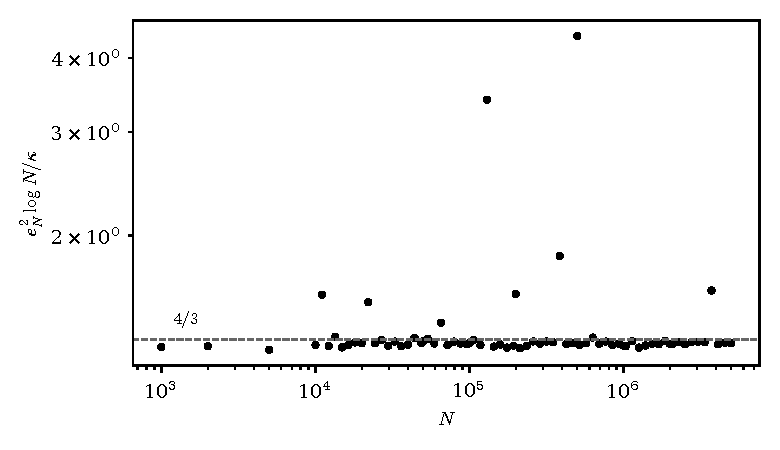
\includegraphics[width=0.78\textwidth]{art1_fig2.pdf}
\caption{$e_N^2\log N/\kappa$ for the two-parameter family of Proposition~\ref{prop:NB}, $998\le N\le5\cdot10^6$ (log scale). Dashed: $4/3$.}\label{fig:NB}
\end{figure}

\section{Numerical checks}\label{sec:num}

These computations check implementations and identities; they are not evidence about $\Theta$ (RH is known up to height $3\cdot10^{12}$~\cite{PT21}).

\emph{Lemmas.} Lemma~\ref{lem:support} agrees with the definition of $c$ for $n\le2\cdot10^4$ (largest discrepancy $7\cdot10^{-15}$); $G(1+10^{-6})=0.2294606$ against $2\gE^2+6\gamma_1=0.2294608$; $h^2G(\rho_1+h)=1.99998-1.6\cdot10^{-6}i$ for $h=10^{-5}$, $\rho_1=\frac12+14.1347\ldots i$.

\emph{The constant $\kappa$.} With the $1070$ zeros of height $\le1500.35$, $2\sum|\rho|^{-2}=0.0448179$; adding the tail $(\pi T)^{-1}(\log(T/2\pi)+1)=0.0013738$ gives $0.0461918$, against $\kappa=0.0461914$ (relative difference $8\cdot10^{-6}$).

\emph{The energy $Q$.} $C$ was computed by a sieve from Lemma~\ref{lem:support} and $Q(X)=\sum_{n<X}C(n)^2(\frac1n-\frac1{n+1})$ for integral $X$; two independent implementations agree to all printed digits up to $10^7$, and one was run to $10^8$. Table~\ref{tab:Q} and Figure~\ref{fig:Q} show the ratio to the leading term. Numerically, $\max_{10^3\le x\le10^8}|C(x)|/(\sqrt x\log^2x)=0.148$.

\begin{table}[h]
\centering\small
\begin{tabular}{rrrrrr}
\toprule
$X$ & $L=\log X$ & $Q(X)$ & $\frac{4\kappa}3L^3$ & ratio & $\log(1+Q)/\log X$\\
\midrule
$10^3$ & 6.908 & 8.936 & 20.30 & 0.440 & 0.332\\
$10^4$ & 9.210 & 27.03 & 48.12 & 0.562 & 0.362\\
$10^5$ & 11.513 & 60.49 & 93.98 & 0.644 & 0.358\\
$10^6$ & 13.816 & 111.34 & 162.41 & 0.686 & 0.342\\
$10^7$ & 16.118 & 186.74 & 257.89 & 0.724 & 0.325\\
$3\cdot10^7$ & 17.217 & 221.82 & 314.30 & 0.706 & 0.314\\
$10^8$ & 18.421 & 290.58 & 384.96 & 0.755 & 0.308\\
\bottomrule
\end{tabular}
\caption{The energy $Q(X)$ and the ratio $Q(X)/(\frac{4\kappa}3\log^3X)$.}\label{tab:Q}
\end{table}

\begin{figure}[t]
\centering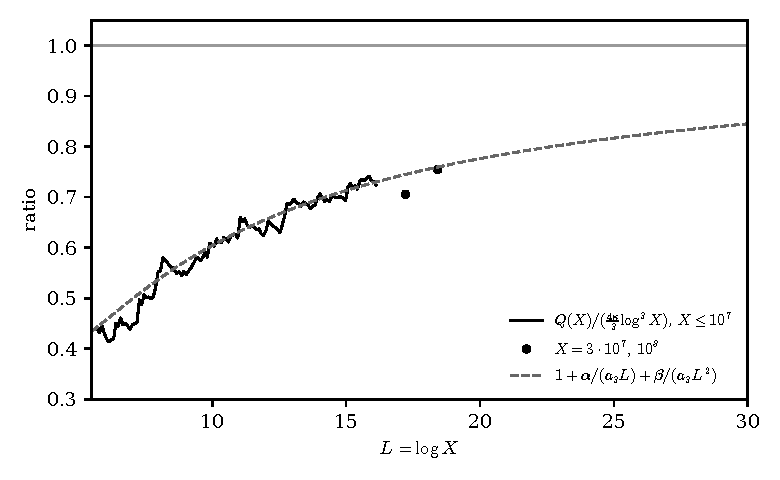
\includegraphics[width=0.78\textwidth]{art1_fig1.pdf}
\caption{Ratio $Q(X)/(\frac{4\kappa}{3}\log^3X)$ for $300\le X\le10^7$ (solid) and at $X=3\cdot10^7,10^8$ (dots), with the heuristic two-term model of Section~\ref{sec:num} (dashed), $a_3=4\kappa/3$.}\label{fig:Q}
\end{figure}

\emph{Why the convergence is slow (heuristic).} Assuming RH and simple zeros, the explicit formula suggests $U(L)=a_3L^3+\alpha L^2+\beta L+L^2\Phi(L)+O(L)$ with $a_3=4\kappa/3$, $\alpha=2\sum_\rho[\Re b_\rho/|\rho|^2-|\rho|^{-4}]$ and $\Phi$ almost periodic of mean zero. For $\rho$ on the critical line, $\Re(\zeta''/\zeta'(\rho))=-2\theta'(\gamma)$, where $\theta$ is the Riemann--Siegel theta function, so $\Re b_\rho=-2\theta'(\gamma)-2\gE$ and $\alpha$ can be computed from the ordinates alone with an analytic tail: $\alpha=-0.3074$, stable from $100$ to $1070$ zeros. The coefficient $\beta\approx0.64$ is less certain (heuristic tail). The resulting model $1+\alpha/(a_3L)+\beta/(a_3L^2)$ predicts $0.717$ at $L=15.2$ (measured $0.723$) and $0.760$ at $L=18.4$ (measured $0.755$); the ratio would reach $0.9$ only near $X\approx10^{21}$. None of this is proved; a remainder term in Theorem~\ref{thm:B} would require uniform control of the off-diagonal terms of Lemma~\ref{lem:loc}, that is, information on close pairs of zeros and on $\zeta'(\rho)$.

\emph{A calibration.} The same computation for the Davenport--Heilbronn function~\cite{DH36}, which satisfies a functional equation but has no Euler product and has zeros off the critical line (the first at $0.8085+85.699i$), gives a fitted growth slope $\log Q/\log X\approx0.56$, against $0.33$ for $\zeta$ and $0.34$ for $L(s,\chi_5)$ over the same range. These finite calibrations show sensitivity in the tested examples. Theorems~\ref{thm:A}--\ref{thm:B} are proved here for $\zeta$; extending them to a general $F$ requires separate analytic bounds and control of its logarithmic derivative and poles.

\section{Open questions}\label{sec:open}

\begin{enumerate}
\item Is Theorem~\ref{thm:B}, or a general Cram\'er-type theorem for Dirichlet series with poles of order $k$ on $\Re s=\frac12$ (giving a logarithmic mean square of order $(\log X)^{2k-1}$), already in the literature?
\item Can one prove $Q(X)=\frac S3(\log X)^3+O((\log X)^{3-\delta})$ under RH alone, or does any rate require a hypothesis on close pairs of zeros or on $\zeta'(\rho)$?
\item Under RH, can one control both $\beta_N\log^2N$ and $T_N\log N$ along a specified sequence on which $A_N$ stays quantitatively away from zero?
\end{enumerate}

\subsection*{Acknowledgements and disclosure}
The original computations and draft used Anthropic's Claude; the two-parameter family of Section~\ref{sec:NB} was first suggested in an exchange with an OpenAI model. The V6.34 audit, revisions and joint criterion, and the V6.36 checks of finite-range and conditional statements, were assisted by OpenAI's ChatGPT. Final mathematical verification and responsibility for submission rest with the author; the note has not been independently refereed. Code and data are available from the author.

\begin{thebibliography}{99}
\bibitem{AF26} L. Alp\"oge, R. Furman, \emph{More than two thirds of the zeros of the Riemann zeta function are simple and on the critical line}, arXiv:2608.13637 (2026).
\bibitem{ANS14} A. Akbary, N. Ng, M. Shahabi, \emph{Limiting distributions of the classical error terms of prime number theory}, Q. J. Math. (2014); arXiv:1306.1657.
\bibitem{Bae03} L. B\'aez-Duarte, \emph{A strengthening of the Nyman--Beurling criterion for the Riemann hypothesis}, Atti Accad. Naz. Lincei Rend. Lincei Mat. Appl. (9) 14 (2003), 5--11.
\bibitem{BCF13} S. Bettin, J. B. Conrey, D. W. Farmer, \emph{An optimal choice of Dirichlet polynomials for the Nyman--Beurling criterion}, Proc. Steklov Inst. Math. 280 (2013); arXiv:1211.5191.
\bibitem{Beu55} A. Beurling, \emph{A closure problem related to the Riemann zeta-function}, Proc. Nat. Acad. Sci. U.S.A. 41 (1955), 312--314.
\bibitem{BPT22} R. P. Brent, D. J. Platt, T. S. Trudgian, \emph{The mean square of the error term in the prime number theorem}, J. Number Theory 238 (2022), 740--762.
\bibitem{BS22} W. D. Banks, S. Sinha, \emph{The Riemann Hypothesis via the generalized von Mangoldt function}, arXiv:2209.11768.
\bibitem{Cra22} H. Cram\'er, \emph{Ein Mittelwertsatz in der Primzahltheorie}, Math. Z. 12 (1922), 147--153.
\bibitem{Dav00} H. Davenport, \emph{Multiplicative Number Theory}, 3rd ed., Springer, 2000.
\bibitem{DH36} H. Davenport, H. Heilbronn, \emph{On the zeros of certain Dirichlet series}, J. London Math. Soc. 11 (1936), 181--185 and 307--312.
\bibitem{GGL20} S. M. Gonek, S. W. Graham, Y. Lee, \emph{The Lindel\"of hypothesis for primes is equivalent to the Riemann hypothesis}, Proc. Amer. Math. Soc. 148 (2020), 2863--2875.
\bibitem{Kor04} J. Korevaar, \emph{Tauberian Theory: A Century of Developments}, Springer, 2004.
\bibitem{Lam26} Y. Lamzouri, \emph{A new proof that more than 2/3 of the zeros of the Riemann zeta function are simple and on the critical line}, arXiv:2609.02882 (2026).
\bibitem{MV07} H. L. Montgomery, R. C. Vaughan, \emph{Multiplicative Number Theory I. Classical Theory}, Cambridge University Press, 2007.
\bibitem{Nym50} B. Nyman, \emph{On the one-dimensional translation group and semi-group in certain function spaces}, Thesis, Uppsala, 1950.
\bibitem{PT21} D. J. Platt, T. S. Trudgian, \emph{The Riemann hypothesis is true up to $3\cdot10^{12}$}, Bull. London Math. Soc. 53 (2021), 792--797.
\bibitem{Tit86} E. C. Titchmarsh, \emph{The Theory of the Riemann Zeta-Function}, 2nd ed., revised by D. R. Heath-Brown, Oxford, 1986.
\bibitem{Wid41} D. V. Widder, \emph{The Laplace Transform}, Princeton University Press, 1941.
\end{thebibliography}

\end{document}
